% =============================================================
%  INTRODUÇÃO
% =============================================================
\section{Introdução}
\label{sec:introducao}

A computação multipartidária segura (\textit{Secure Multiparty Computation}, SMC) permite que duas ou mais partes calculem em conjunto uma função sobre os seus dados privados sem que nenhuma delas tenha de revelar à outra os seus inputs. Um caso particular com inúmeras aplicações práticas é a \textit{Private Set Intersection} (PSI), em que cada parte detém um conjunto de elementos e pretende descobrir apenas a intersecção desses conjuntos, sem expor os restantes elementos.

Este trabalho explora, na prática, quatro protocolos de PSI implementados na biblioteca \textit{PSI} do grupo ENCRYPTO da TU Darmstadt~\cite{psi_repo}: \emph{naive hashing}, \emph{server-aided}~\cite{kamara2014scaling}, \emph{Diffie-Hellman}~\cite{meadows1986matchmaking} e \emph{OT-based}~\cite{pinkas2014faster, pinkas2016scalable}. O relatório está organizado em torno dos quatro passos definidos no enunciado: a Secção~\ref{sec:step1} descreve e compara os protocolos; a Secção~\ref{sec:step2} reporta a experimentação com inputs simples e com listas de aplicações móveis, complementada por captura de pacotes em Wireshark e por uma análise crítica das propriedades de segurança e custo de comunicação; a Secção~\ref{sec:step3} apresenta benchmarks de tempo e dados trocados em função do tamanho dos conjuntos; e a Secção~\ref{sec:step4} aplica PSI a um caso de uso real entre os autores. O relatório encerra na Secção~\ref{sec:conclusao} com uma discussão integrada dos resultados.


% =============================================================
%  STEP 1: PROTOCOLOS DE PSI
% =============================================================
\section{Protocolos de Private Set Intersection: Estudo e Comparação}
\label{sec:step1}

\subsection{Naive Hashing}
\label{sec:naive}

O \emph{naive hashing} é a abordagem mais simples para PSI e parte de uma ideia directa: se duas partes aplicarem a mesma função de hash criptográfica aos elementos dos seus conjuntos e trocarem entre si as listas de hashes resultantes, qualquer hash que apareça em ambas as listas corresponde, com probabilidade esmagadora, a um elemento comum~\cite{pinkas2016scalable}. Cada parte $P_i$ com conjunto $S_i$ calcula $H(x)$ para todo $x \in S_i$, envia o conjunto de hashes à contraparte e determina a intersecção comparando hashes recebidos com os locais. O elemento original é depois recuperado a partir da pré-imagem que ficou guardada no lado de quem hashou.

Na implementação da biblioteca usada neste trabalho, $H$ é SHA-256 truncado aos primeiros bytes (por omissão 6 bytes, ou seja 48 bits, configurável via \texttt{-b}). Esta truncagem foi adoptada por motivos de eficiência: reduz o volume transmitido em mais de cinco vezes face ao output completo de 256 bits e a probabilidade residual de colisões mantém-se aceitável para conjuntos pequenos. A consequência, discutida na Secção~\ref{sec:disc_naive}, é o agravamento da vulnerabilidade a ataques de pré-imagem.

Em termos de custos, o protocolo é assimptoticamente óptimo: a comunicação é $O(n)$ hashes por parte e a computação resume-se a $n$ avaliações de SHA-256 em cada lado, sem operações de chave pública nem rondas adicionais para além da troca das duas listas. Não há partilha de segredos prévios nem assunções criptográficas para além da resistência a colisões e a pré-imagens da função de hash, o que torna o naive hashing a baseline natural contra a qual todos os protocolos PSI mais robustos são comparados~\cite{pinkas2016scalable}. É também usado, na sua forma directa, em produção por aplicações como Signal ou Secret para descoberta de contactos, sempre que o contexto permite assumir um domínio de inputs com entropia suficiente.

\subsection{Server-Aided (Kamara et al.)}
\label{sec:serveraided}

O protocolo \emph{server-aided} de Kamara et al.~\cite{kamara2014scaling} introduz um terceiro participante, um servidor externo, com o objectivo de delegar nele o esforço computacional da intersecção sem lhe entregar os dados em claro. O modelo de confiança é semi-honesto e exige a hipótese de \textbf{não-colusão}: assume-se que o servidor segue correctamente o protocolo e que não conspira com nenhuma das partes, embora possa tentar inferir informação a partir do que recebe. Esta hipótese é geralmente justificada por incentivos legais e reputacionais e é o que distingue o modelo do server-aided puro de uma terceira parte plenamente confiável.

Operacionalmente, as duas partes acordam previamente uma chave secreta $K$ para uma \emph{pseudorandom permutation} (PRP) $F_K$. Cada parte $P_i$ com conjunto $S_i$ calcula $\pi_i(F_K(S_i))$, isto é, aplica a PRP a todos os elementos e permuta aleatoriamente o resultado para esconder a ordem original. Os conjuntos pseudoaleatórios assim produzidos são enviados ao servidor, que executa a intersecção em tempo linear sobre os valores recebidos e devolve a intersecção (no espaço da PRP) às partes. Cada uma aplica $F_K^{-1}$ aos elementos devolvidos para recuperar a intersecção em claro~\cite{kamara2014scaling}. O servidor nunca tem acesso à chave $K$ nem aos conjuntos originais, e os elementos que vê são, sob a hipótese de PRP, indistinguíveis de valores aleatórios.

A grande vantagem reside na escalabilidade: o protocolo foi desenhado e testado para conjuntos da ordem dos biliões de elementos, com o tempo total apenas cerca de 10\% superior ao de uma intersecção em claro, dado que tanto o lado dos clientes (avaliações de PRP) como o do servidor (intersecção sobre uma tabela de hash) são lineares em $n$~\cite{kamara2014scaling}. Para reforçar o protocolo contra um servidor potencialmente malicioso, os autores propõem ainda introduzir repetições controladas dos elementos e \emph{dummies} estruturados, cujo desaparecimento na resposta do servidor permite detectar manipulação com probabilidade negligenciável. As principais limitações são, naturalmente, a confiança depositada na ausência de colusão e a introdução de um ponto único de falha que não existia no modelo de duas partes.

\subsection{Diffie-Hellman PSI (Meadows)}
\label{sec:dh}

O protocolo de Meadows~\cite{meadows1986matchmaking}, originalmente proposto como \emph{cryptographic matchmaking}, foi a primeira construção de PSI puramente entre duas partes sem recurso a um terceiro durante a execução, e baseia-se na comutatividade da exponenciação modular. As partes A e B acordam um grupo cíclico de ordem prima onde o problema do logaritmo discreto é difícil, e cada uma escolhe um expoente secreto, $a$ e $b$ respectivamente. Os elementos do conjunto são primeiro projectados no grupo através de uma função de hash $H$ que actua como random oracle.

A execução decorre em duas trocas. Numa primeira ronda, cada parte envia à outra os seus elementos elevados ao expoente próprio: A envia $\{H(x_i)^{a}\}$ e B envia $\{H(y_j)^{b}\}$. Numa segunda ronda, cada parte eleva os valores recebidos ao seu próprio expoente, obtendo $H(y_j)^{ba}$ no lado de A e $H(x_i)^{ab}$ no lado de B, e devolve esses valores. Pela comutatividade da exponenciação, $H(x)^{ab} = H(x)^{ba}$, pelo que cada parte consegue comparar localmente os duplamente-exponenciados que possui com os que recebe da contraparte e, sempre que houver coincidência, conclui que esse elemento pertence à intersecção sem nunca aprender qualquer outro elemento da contraparte. A segurança contra um adversário semi-honesto reduz-se à hipótese decisional de Diffie-Hellman (DDH) no grupo escolhido: sem o expoente secreto da contraparte, $H(x)^{a}$ é indistinguível de um elemento aleatório do grupo.

A versão original, contudo, oferece apenas garantias contra adversários honestos, pois uma das partes pode forjar uma correspondência inserindo valores arbitrários do grupo. Para mitigar este risco, Meadows propõe operar no grupo multiplicativo $\mathbb{Z}_N^*$ com $N=(2pq+1)(2r+1)$, ancorando a segurança na dificuldade da factorização e exigindo que cada parte autentique os seus pontos com assinaturas digitais; conhecer $\phi(N)=4pqr$ seria computacionalmente equivalente a quebrar RSA, o que torna inviável a forja~\cite{meadows1986matchmaking}. Em termos de custos, o protocolo exige $2n$ exponenciações modulares por parte e a comunicação consiste em $O(n)$ elementos do grupo, dimensão que tipicamente excede em cerca de uma ordem de grandeza a de um hash truncado. É esta combinação de exponenciações por elemento que, como se verá no Step~3, domina o tempo total e limita a escalabilidade do protocolo para conjuntos grandes.

\subsection{OT-Based PSI (Pinkas, Schneider, Zohner)}
\label{sec:ot}

O protocolo baseado em \emph{Oblivious Transfer} de Pinkas, Schneider e Zohner~\cite{pinkas2014faster, pinkas2016scalable} substitui as operações de chave pública das construções anteriores por primitivas simétricas, recorrendo a OT extension para reduzir drasticamente o custo computacional. A primitiva central é uma \emph{Oblivious Pseudorandom Function} (OPRF): o servidor detém uma chave secreta $k$, o cliente possui um input $x$, e a OPRF permite ao cliente obter $F_k(x)$ sem aprender $k$ e sem que o servidor aprenda $x$. Avaliada esta função sobre os elementos de ambos os conjuntos, a intersecção reduz-se a comparar os outputs da OPRF.

Para tornar o protocolo escalável, os autores combinam três técnicas. Primeiro, o cliente distribui os seus elementos por uma tabela de \emph{Cuckoo hashing} com $k$ funções de hash, garantindo que cada elemento ocupa um único bin com alta probabilidade; em paralelo, o servidor distribui os seus elementos por \emph{simple hashing} sobre a mesma estrutura, replicando cada elemento em todos os bins indicados pelas $k$ funções e introduzindo \emph{dummies} para mascarar o número real de elementos por bin. Segundo, para evitar colisões prematuras entre elementos atribuídos ao mesmo bin por funções diferentes, é usada uma representação baseada em permutação que codifica também o índice da função de hash que mapeou o elemento. Terceiro, a avaliação das OPRFs em todos os bins é feita em paralelo através de \emph{$\binom{N}{1}$-OT extension}: para cada bin com índice $i$, o servidor escolhe uma chave $t_i$, avalia a PRF localmente sobre os seus elementos desse bin e desempenha o papel de remetente num OT em que o cliente, como receptor, recebe apenas a avaliação correspondente ao seu próprio elemento, sem aprender as restantes nem a chave $t_i$. As máscaras resultantes do servidor são permutadas e enviadas ao cliente, que as compara com as que calculou localmente.

A robustez do protocolo contra falsos positivos depende da escolha do comprimento da máscara $\ell = \lambda + \log_2(kn_1) + \log_2(n_2)$, onde $\lambda$ é o parâmetro estatístico de segurança e $n_1$, $n_2$ os tamanhos dos conjuntos: este valor garante que a probabilidade de colisão entre máscaras de elementos distintos é no máximo $2^{-\ell}$ e, consequentemente, que o protocolo retorna a intersecção correcta com probabilidade pelo menos $1 - 2^{-\lambda}$~\cite{pinkas2016scalable}. Em termos de custos, a comunicação é dominada pela fase de OT extension e cresce como $O(n\,\ell)$ bits, mas inclui um overhead inicial fixo independente de $n$ correspondente às base OTs; o custo computacional é quase linear e baseia-se quase inteiramente em primitivas simétricas. Esta combinação coloca o protocolo entre os mais escaláveis para PSI semi-honesto e justifica que, como se verá no Step~3, o tempo de execução se mantenha praticamente constante até $10^5$ elementos.

\subsection{Comparação Resumida}
\label{sec:comparacao}

Os quatro protocolos descritos representam pontos distintos no espaço de compromissos entre eficiência, escalabilidade, garantias de segurança e modelo de confiança. A discussão que se segue articula os trade-offs que justificam a escolha de cada protocolo em diferentes contextos práticos.

O \emph{naive hashing} é, por construção, o mais simples e o mais eficiente em termos computacionais e de comunicação, várias ordens de grandeza mais rápido do que os protocolos criptograficamente seguros~\cite{pinkas2016scalable}. A sua segurança depende inteiramente da entropia do domínio dos inputs: para conjuntos com elementos previsíveis ou com domínio público, é trivial montar ataques de dicionário ou de pré-imagem, especialmente quando o hash é truncado. Esta fragilidade é particularmente relevante neste trabalho, em que os domínios usados (nomes de aplicações Android, Track IDs do Spotify, números mecanográficos) são todos públicos e enumeráveis.

O protocolo \emph{server-aided} oferece a melhor escalabilidade absoluta, com desempenho próximo do de uma intersecção em claro mesmo para conjuntos da ordem dos biliões~\cite{kamara2014scaling}, à custa de delegar a computação num terceiro semi-honesto não conluiado. A hipótese de não-colusão é forte e o protocolo herda, em essência, a mesma fragilidade do naive hashing perante o servidor (que vê valores deterministicamente derivados dos inputs), pelo que o seu uso só se justifica quando os ganhos de escalabilidade compensam a introdução de um terceiro com incentivos credíveis para se comportar honestamente.

O protocolo baseado em \emph{Diffie-Hellman} é o mais antigo e o mais simples conceptualmente entre os criptograficamente seguros, sem necessitar de terceiros após a fase de inicialização~\cite{meadows1986matchmaking}. A sua segurança ancora-se em problemas bem estudados (DDH e, na variante reforçada, factorização) e a implementação é compacta, mas o custo de $2n$ exponenciações modulares por parte degrada-se rapidamente com $n$, tornando-o inadequado para conjuntos grandes. É, no entanto, competitivo para aplicações com poucos elementos onde a simplicidade e a ausência de terceiros sejam vantagens decisivas.

Por fim, o protocolo baseado em \emph{Oblivious Transfer} é o mais robusto e versátil, oferecendo segurança contra adversários semi-honestos com extensões para o modelo malicioso, e mantendo um tempo de execução praticamente constante para uma vasta gama de tamanhos graças ao recurso a OPRFs e OT extension. A contrapartida é uma maior complexidade de implementação e um overhead fixo de comunicação que penaliza conjuntos pequenos, mas que se amortiza rapidamente à medida que $n$ cresce. É, na prática, o protocolo de eleição quando se exige privacidade rigorosa e capacidade de lidar com grandes volumes de dados.



% =============================================================
%  STEP 2: EXPERIMENTAÇÃO
% =============================================================
\section{Experimentação com os Protocolos}
\label{sec:step2}

Esta secção reporta a execução prática dos quatro protocolos sobre inputs controlados (pontos 1--4) e sobre as listas \texttt{AppList1.csv} e \texttt{AppList2.csv} fornecidas com o enunciado (pontos 5--10). Todas as experiências foram realizadas localmente, com captura de tráfego em Wireshark sobre a interface \texttt{loopback} e filtro \texttt{tcp.port == 7766}.

\subsection{Naive Hashing com Inputs Simples (pontos 1--3)}
\label{sec:naive_simples}

Foi criado o ficheiro \texttt{input} com o número mecanográfico \texttt{up202509273} e o ficheiro \texttt{input2} com a palavra \texttt{test}. Os hashes esperados, obtidos por SHA-256 truncado a 6 bytes, são:

\begin{itemize}
  \item \texttt{up202509273} $\rightarrow$ \texttt{478ed603b634}
  \item \texttt{test} $\rightarrow$ \texttt{9f86d081884c}
\end{itemize}

Verificação manual: \texttt{echo -n up202509273 | sha256sum | cut -c -12} produz \texttt{478ed603b634}, confirmando o algoritmo usado pela biblioteca.

\textbf{Ponto 1.} Com ambos os terminais a usar \texttt{input}, o output foi \texttt{Found 1 intersecting elements: up202509273} e os dois hashes trocados nos sockets coincidiram.

\textbf{Ponto 2.} Com \texttt{input} contra \texttt{input2}, os hashes trocados são distintos e o output foi \texttt{Found 0 intersecting elements}.

\textbf{Ponto 3.} As duas execuções foram repetidas com captura em Wireshark, com filtro \texttt{tcp.port == 7766}. A primeira captura contém 35 pacotes (3\,968 bytes) e o hash \texttt{478ed603b634} aparece duas vezes, uma em cada direção, transportado como payload de um único segmento TCP de 6 bytes em cada sentido. A segunda captura contém 30 pacotes (3\,508 bytes), com cada hash (\texttt{478ed603b634} de um lado e \texttt{9f86d081884c} do outro) a aparecer uma única vez em direções opostas, confirmando que apenas os hashes truncados são trocados pela rede e que coincidem exactamente com os impressos pelo programa nas Figuras~\ref{fig:naive_ex1} e~\ref{fig:naive_ex2}.

\begin{figure}[H]
\centering
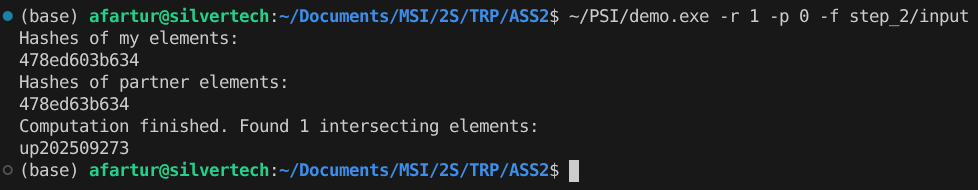
\includegraphics[width=0.85\textwidth]{pictures/naive_ex1_intersect.png}
\caption{Output do protocolo Naive Hashing com ambos os terminais a usar \texttt{input}: os hashes locais e remotos coincidem (\texttt{478ed603b634}) e a intersecção contém o elemento \texttt{up202509273}.}
\label{fig:naive_ex1}
\end{figure}

\begin{figure}[H]
\centering
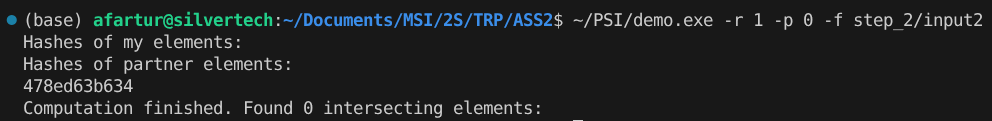
\includegraphics[width=0.85\textwidth]{pictures/naive_ex2_no_intersect.png}
\caption{Output do protocolo Naive Hashing com \texttt{input} contra \texttt{input2}: os hashes locais (\texttt{478ed603b634}) e remotos (\texttt{9f86d081884c}) diferem e a intersecção é vazia.}
\label{fig:naive_ex2}
\end{figure}

\begin{figure}[H]
\centering
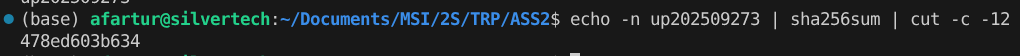
\includegraphics[width=0.85\textwidth]{pictures/naive_sha256_verify.png}
\caption{Verificação manual com \texttt{echo -n up202509273 | sha256sum | cut -c -12}: o resultado \texttt{478ed603b634} confirma que a biblioteca aplica SHA-256 truncado aos primeiros 6 bytes.}
\label{fig:naive_sha256}
\end{figure}

\begin{figure}[H]
\centering
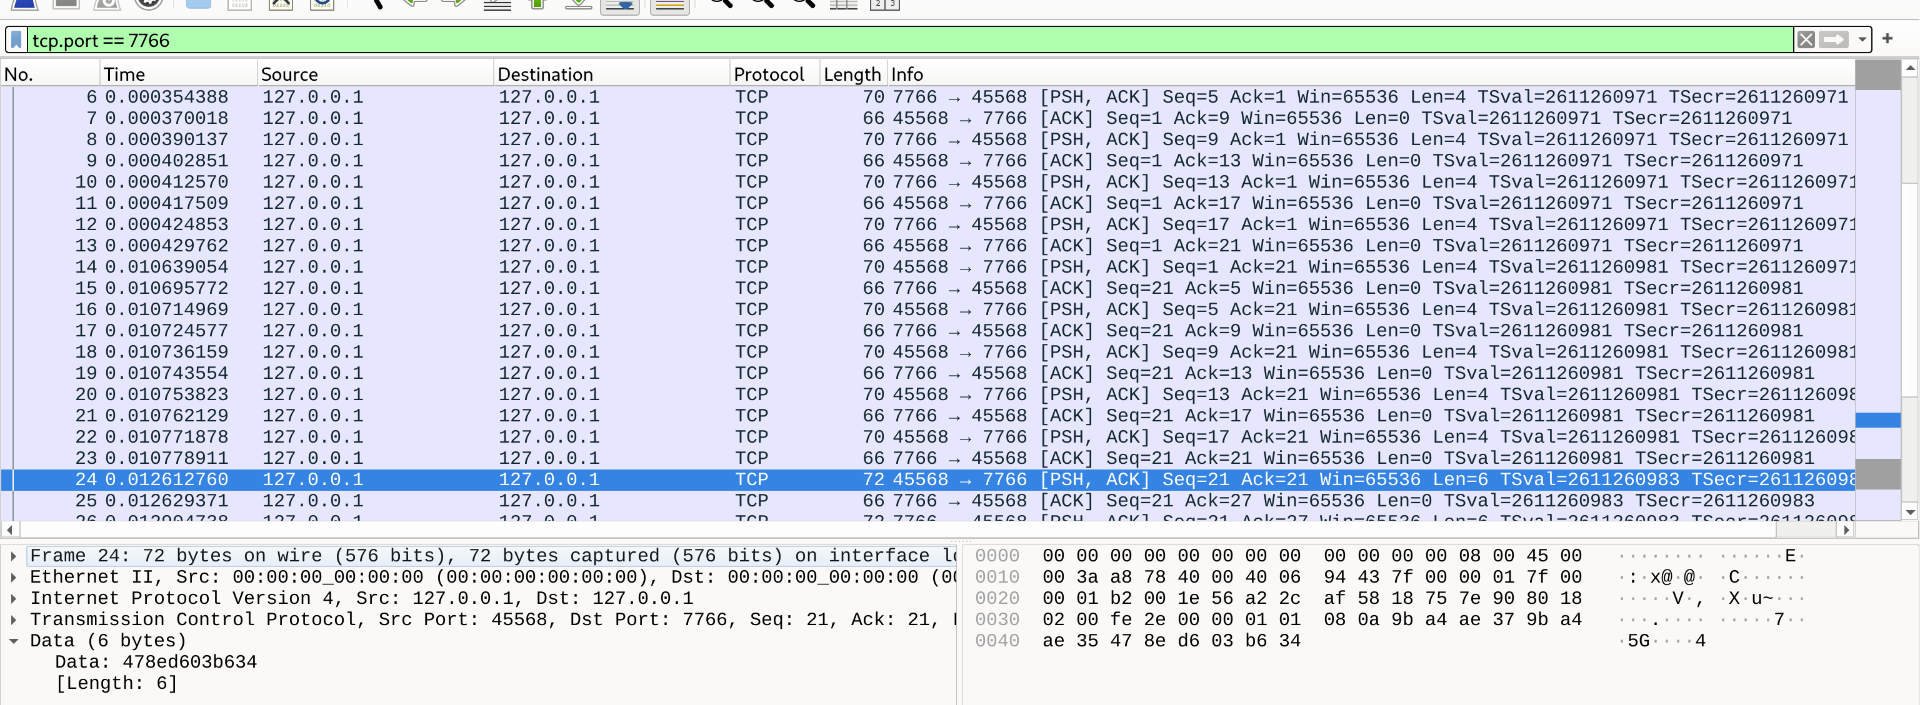
\includegraphics[width=0.95\textwidth]{pictures/wireshark_naive.png}
\caption{Captura Wireshark de um segmento TCP da execução do naive hashing (filtro \texttt{tcp.port == 7766}). O painel inferior mostra o campo \texttt{Data} com os 6 bytes \texttt{478ed603b634} a circular em claro entre as duas partes, idênticos ao hash impresso pelo programa na Figura~\ref{fig:naive_ex1}.}
\label{fig:wireshark_naive}
\end{figure}

\subsection{Discussão: Insegurança do Naive Hashing (ponto 4)}
\label{sec:disc_naive}

A simplicidade que torna o naive hashing eficiente é também a origem das suas falhas de segurança. A função de hash usada é determinística e pública, sem qualquer segredo partilhado entre as partes, pelo que qualquer observador com acesso aos hashes trocados (incluindo a contraparte ou um atacante na rede) pode verificar trivialmente se um candidato concreto $x$ pertence a um dos conjuntos: basta calcular $H(x)$ localmente e procurar o resultado na lista observada. Este facto é directamente visível na captura Wireshark da Figura~\ref{fig:wireshark_naive}, onde os 6 bytes \texttt{478ed603b634} aparecem como payload TCP em claro num único segmento, e correspondem exactamente ao hash que o programa imprime na Figura~\ref{fig:naive_ex1}; como esses bytes são a saída de SHA-256 aplicada respectivamente a \texttt{up202509273} e a \texttt{test}, a re-identificação dos inputs reduz-se a uma simples consulta numa tabela pré-computada. A privacidade do protocolo fica assim reduzida à dificuldade de adivinhar o input, o que para domínios pequenos ou enumeráveis é um problema desprezável.

O agravamento desta fragilidade é duplo. Por um lado, a implementação trunca o output de SHA-256 a apenas 6 bytes (48 bits), reduzindo drasticamente o espaço efectivo de saída e facilitando ataques de pré-imagem por força bruta dentro de qualquer domínio razoavelmente delimitado. Por outro lado, o atacante não precisa sequer de força bruta no espaço completo: para domínios públicos como o conjunto de aplicações Android disponíveis na Play Store, números mecanográficos da FCUP ou identificadores de faixas musicais do Spotify, basta enumerar os candidatos legítimos e pré-computar a tabela de hashes correspondente. Aplicado às listas \texttt{AppList1.csv} e \texttt{AppList2.csv} do ponto 5, este ataque é trivial e revela imediatamente a totalidade das aplicações instaladas em cada lado, e não apenas as cinco da intersecção.

A consequência mais grave é que cada parte não recebe apenas a intersecção: recebe a lista completa de hashes da contraparte. Quando o domínio dos elementos é público, isto é, em termos de privacidade, equivalente a receber o conjunto inteiro em claro, uma vez que cada hash pode ser revertido em tempo desprezável por simples consulta a uma tabela pré-computada. O protocolo viola assim o princípio fundamental de PSI (cada parte deve aprender exclusivamente a intersecção e nada mais), pelo que, apesar da sua eficiência, é inadequado em qualquer cenário onde a confidencialidade dos elementos fora da intersecção tenha de ser preservada.

\subsection{Naive sobre AppList1 vs AppList2 (ponto 5)}
\label{sec:naive_apps}

A intersecção computada com naive hashing contém 5 elementos:
\begin{itemize}\itemsep0pt
  \item \texttt{com.whatsapp}
  \item \texttt{org.meowcat.edxposed.manager}
  \item \texttt{com.google.android.apps.maps}
  \item \texttt{com.android.chrome}
  \item \texttt{com.delaware.empark}
\end{itemize}

A captura Wireshark associada regista 31 pacotes e 4\,016 bytes capturados (2\,613 bytes de payload).

\subsection{Server-Aided (ponto 6)}
\label{sec:srv_aided}

O protocolo \texttt{-p 1} exige que ambas as listas tenham o mesmo número de linhas. Como \texttt{AppList2} (34 entradas) é menor que \texttt{AppList1} (36), foi feito \emph{padding} de \texttt{AppList2} com 2 emails fictícios extraídos da \emph{sample} \texttt{emails\_alice.txt} fornecida com a biblioteca. A execução requer três terminais: o servidor (\texttt{-r 0}), que orquestra o protocolo, e dois clientes (\texttt{-r 1}), cada um com uma das listas paddadas. O servidor reporta \texttt{Connections with all 2 clients established} e termina com \texttt{sending all 5 intersecting elements to the clients}, enquanto cada cliente imprime a intersecção localmente, conforme ilustrado na Figura~\ref{fig:step2_server_aided}. A captura Wireshark associada regista 32 pacotes e 4\,768 bytes capturados (3\,330 bytes de payload).

\begin{figure}[H]
\centering
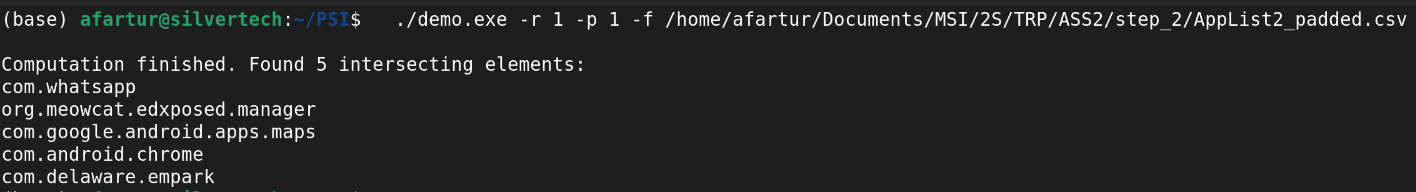
\includegraphics[width=0.95\textwidth]{pictures/step2_server_aided.png}
\caption{Output do cliente do protocolo Server-Aided sobre \texttt{AppList1\_padded.csv} e \texttt{AppList2\_padded.csv}: o terminal mostra a intersecção dos 5 elementos comuns devolvida pelo servidor.}
\label{fig:step2_server_aided}
\end{figure}

\subsection{Discussão: Privacidade do Servidor Third-Party (ponto 7)}
\label{sec:disc_serveraided}

A introdução de um terceiro participante no protocolo server-aided altera substancialmente o modelo de privacidade do PSI e introduz problemas que não existem no cenário estritamente de duas partes. O primeiro problema é estrutural: o servidor recebe, neste protocolo, uma representação dos elementos de ambos os clientes para conseguir computar a intersecção. A construção teórica de Kamara et al.~\cite{kamara2014scaling} assume que essa representação é a saída de uma PRP com chave secreta partilhada apenas entre as partes, indistinguível de aleatório do ponto de vista do servidor. A implementação fornecida pela biblioteca, contudo, transmite ao servidor valores muito próximos dos hashes do protocolo naive: o volume capturado para a execução server-aided (32 pacotes, 4\,768 bytes) é apenas marginalmente superior ao do naive (31 pacotes, 4\,016 bytes) sobre as mesmas listas, indicando que pouca aleatorização adicional é introduzida sobre os elementos antes do envio. O servidor herda assim, em larga medida, a fragilidade discutida na Secção~\ref{sec:disc_naive}: dado que o domínio dos elementos das listas é público e enumerável, basta-lhe pré-computar a transformação aplicada pelos clientes para os candidatos plausíveis e comparar com os valores recebidos, recuperando os elementos originais sem necessidade de quebrar a função de hash subjacente.

A consequência prática deste detalhe de implementação é que a confiança depositada no servidor passa a ser quase total. Ainda que o modelo formal o classifique como semi-honesto, basta uma situação de colusão com uma das partes (ou um comprometimento isolado do servidor) para que toda a lista da contraparte seja reconstruída em claro: na presença do conjunto de uma das partes, o servidor pode pré-computar a tabela $\{H(x) : x \in \mathcal{D}\}$ no domínio relevante e mapear, sem ambiguidade, todos os hashes recebidos da outra parte. Mesmo sem colusão, o servidor aprende sempre o tamanho dos conjuntos, o tamanho da intersecção e os hashes em si, o que para domínios públicos é, conforme já argumentado, equivalente a aprender os elementos.

Por fim, há um custo arquitectural que não desaparece nem com uma escolha mais cuidadosa de primitivas: a introdução do servidor cria um ponto único de falha que, num cenário 2-party puro, simplesmente não existia. Esse ponto centraliza riscos de disponibilidade (negação de serviço, falhas operacionais), de comprometimento (um atacante que controle o servidor controla a privacidade de todas as partes que dele dependam) e mesmo legais (o servidor passa a ser alvo natural para pedidos de divulgação compulsiva). O ganho do protocolo está, portanto, exclusivamente na escalabilidade, ao reduzir a interacção a uma ronda cliente-servidor em vez das múltiplas rondas e exponenciações de protocolos como o de Diffie-Hellman, e não em garantias adicionais de privacidade. A sua adopção só se justifica quando essa hipótese de confiança é credível e os ganhos de desempenho compensam efectivamente os riscos introduzidos.

\subsection{Diffie-Hellman PSI (ponto 8)}
\label{sec:exp_dh}

A intersecção devolvida contém os mesmos 5 elementos do naive. No protocolo DH, apenas o terminal com \texttt{-r 1} computa e imprime a intersecção, conforme se observa na Figura~\ref{fig:step2_dh}. A captura associada regista 30 pacotes e 7\,084 bytes capturados (5\,714 bytes de payload). O aumento face ao naive deve-se à transmissão de elementos de grupo (em vez de hashes truncados) e ao handshake DH.

\begin{figure}[H]
\centering
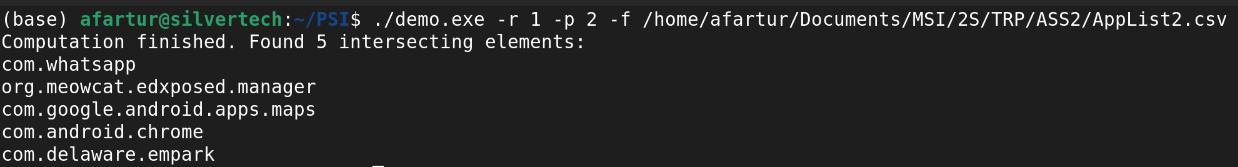
\includegraphics[width=0.95\textwidth]{pictures/step2_dh.png}
\caption{Output do cliente (\texttt{-r 1}) do protocolo Diffie-Hellman sobre \texttt{AppList1.csv} e \texttt{AppList2.csv}.}
\label{fig:step2_dh}
\end{figure}

\subsection{OT-Based PSI (ponto 9)}
\label{sec:exp_ot}

A intersecção coincide novamente com a do naive. A captura associada regista 36 pacotes e 56\,580 bytes capturados (55\,006 bytes de payload). O custo é dominado pela fase de \emph{base OTs} e \emph{OT extension}, cujo overhead é praticamente independente de $n$ para conjuntos pequenos. A Figura~\ref{fig:step2_ot} mostra o output do cliente, onde além da intersecção é possível ver a configuração concreta do protocolo (34 elementos hashados em palavras de 7 bytes, 41 \emph{bins} e 41 OTs efectuadas, com \texttt{maskbitlen = 56}). É também notório o aviso \texttt{Insertion not successful for element 30!}, indicando que a inserção de um dos elementos no Cuckoo hashing falhou no número configurado de tentativas e foi tratada via mecanismo de \emph{stash}, sem afectar a correcção do resultado.

\begin{figure}[H]
\centering
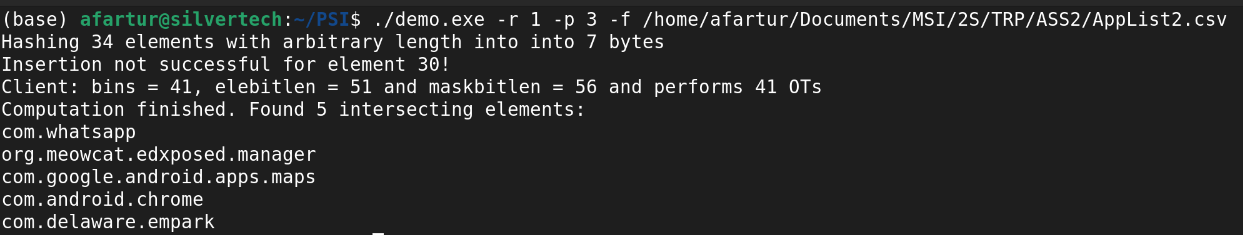
\includegraphics[width=0.95\textwidth]{pictures/step2_ot.png}
\caption{Output do cliente (\texttt{-r 1}) do protocolo OT-based sobre \texttt{AppList1.csv} e \texttt{AppList2.csv}.}
\label{fig:step2_ot}
\end{figure}

\subsection{Análise Comparativa Segurança vs Custo de Comunicação (ponto 10)}
\label{sec:disc_comm_cost}

\begin{table}[H]
\centering
\caption{Pacotes e bytes capturados em Wireshark para os quatro protocolos sobre as listas de apps.}
\label{tab:step2_pktbytes}
\begin{tabular}{lcc}
\toprule
\textbf{Protocolo} & \textbf{Pacotes} & \textbf{Bytes capturados} \\
\midrule
Naive hashing (-p 0)        & 31 & 4\,016 \\
Server-aided (-p 1)         & 32 & 4\,768 \\
Diffie-Hellman (-p 2)       & 30 & 7\,084 \\
OT-based (-p 3)             & 36 & 56\,580 \\
\bottomrule
\end{tabular}
\end{table}

A Tabela~\ref{tab:step2_pktbytes} torna visível um compromisso recorrente entre custo de comunicação e nível de segurança que cada protocolo oferece. A leitura conjunta destes valores com as discussões dos pontos 4 e 7 permite caracterizar a posição de cada protocolo no espaço deste compromisso.

O \emph{naive hashing} é o mais barato em pacotes e bytes (4\,016 bytes), o que se compreende: cada parte envia apenas $n$ hashes truncados de 6 bytes, sem qualquer ronda adicional. Esse custo mínimo, no entanto, está directamente ligado às fragilidades discutidas anteriormente, uma vez que é precisamente a ausência de aleatorização e de chave secreta que permite a representação compacta. O protocolo só é tolerável em cenários onde o domínio dos elementos seja suficientemente grande e imprevisível para tornar inviáveis os ataques de dicionário, o que raramente se verifica em casos práticos como aplicações instaladas, contactos ou identificadores em catálogos públicos.

O \emph{server-aided} apresenta um custo apenas marginalmente superior ao naive (4\,768 bytes, 32 pacotes). Esse acréscimo é coerente com a introdução de um terceiro participante e de uma ronda extra para devolver a intersecção, mas é demasiado pequeno para ser compatível com qualquer transformação criptográfica robusta dos elementos antes do envio. Como discutido na Secção~\ref{sec:disc_serveraided}, o protocolo essencialmente substitui a partilha bilateral de hashes pela centralização desses mesmos hashes num servidor, trocando uma vulnerabilidade por outra sem que a privacidade efectiva melhore.

O protocolo baseado em \emph{Diffie-Hellman} paga aproximadamente 75\% mais bytes do que o naive (7\,084 bytes) por transmitir elementos de um grupo cíclico em vez de hashes truncados, e por exigir duas rondas de troca para concretizar a comutatividade. Em troca, elimina por completo a vulnerabilidade a ataques de dicionário, uma vez que cada elemento é mascarado por um expoente secreto da contraparte. O custo de comunicação cresce, portanto, em proporção directa ao ganho de segurança, e o overhead na ordem dos kilobytes é facilmente absorvido em qualquer ligação moderna.

O protocolo baseado em \emph{Oblivious Transfer} apresenta o maior custo absoluto, com 56\,580 bytes capturados, cerca de uma ordem de grandeza acima dos restantes. Este valor é, em larga medida, um custo fixo de inicialização: a fase de \emph{base OTs} e a montagem do canal de \emph{OT extension} têm um overhead independente de $n$ que para conjuntos pequenos como o destes 36 elementos domina o total transmitido. O Step~3 confirmará que esse custo se amortiza rapidamente à medida que $n$ cresce e que, em contrapartida, o tempo de execução se mantém praticamente constante, o que faz deste protocolo a melhor escolha para conjuntos grandes apesar de ser o pior para conjuntos pequenos.

Em síntese, observa-se uma clara monotonia entre garantia de segurança e custo de comunicação: cada salto qualitativo (de hashes em claro para mascaramento por expoentes secretos, e destes para OPRFs avaliadas via OT) corresponde a um aumento mensurável no volume de bytes trocados. Para conjuntos pequenos sobre domínios públicos, nenhum protocolo é simultaneamente barato e seguro, e a decisão depende sempre da relação entre o valor da informação a proteger e os recursos disponíveis para o protocolo.


% =============================================================
%  STEP 3: BENCHMARKING
% =============================================================
\section{Benchmarking de Protocolos PSI}
\label{sec:step3}

Foi escrito um script de benchmark que executa \texttt{psi.exe} para cada combinação de protocolo $\in \{0, 2, 3\}$ e $n \in \{50, 100, 500, 1\,000, 5\,000, 10\,000, 50\,000, 100\,000\}$, com \texttt{-b 16}, registando tempo, dados enviados e dados recebidos do lado do cliente (\texttt{-r 1}). O protocolo 1 (server-aided) foi excluído por instabilidade documentada na biblioteca.

\subsection{Resultados}
\label{sec:bench_results}

\begin{table}[H]
\centering
\caption{Benchmarks de tempo e dados trocados (\texttt{psi.exe -b 16}).}
\label{tab:bench}
\renewcommand{\arraystretch}{1.15}
\begin{tabular}{lrrrrr}
\toprule
\textbf{Protocolo} & \textbf{n} & \textbf{Tempo (s)} & \textbf{Sent (MB)} & \textbf{Recv (MB)} & \textbf{Total (MB)} \\
\midrule
Naive (0) & 50      & 0.0  & 0.0 & 0.0 & 0.0 \\
Naive (0) & 100     & 0.0  & 0.0 & 0.0 & 0.0 \\
Naive (0) & 500     & 0.0  & 0.0 & 0.0 & 0.0 \\
Naive (0) & 1\,000  & 0.0  & 0.0 & 0.0 & 0.0 \\
Naive (0) & 5\,000  & 0.0  & 0.0 & 0.0 & 0.0 \\
Naive (0) & 10\,000 & 0.0  & 0.1 & 0.1 & 0.2 \\
Naive (0) & 50\,000 & 0.1  & 0.4 & 0.4 & 0.8 \\
Naive (0) & 100\,000 & 0.3 & 1.0 & 1.0 & 2.0 \\
\midrule
DH (2)    & 50      & 0.0  & 0.0 & 0.0 & 0.0 \\
DH (2)    & 100     & 0.0  & 0.0 & 0.0 & 0.0 \\
DH (2)    & 500     & 0.2  & 0.0 & 0.0 & 0.0 \\
DH (2)    & 1\,000  & 0.4  & 0.0 & 0.1 & 0.1 \\
DH (2)    & 5\,000  & 2.1  & 0.2 & 0.3 & 0.5 \\
DH (2)    & 10\,000 & 4.3  & 0.4 & 0.7 & 1.1 \\
DH (2)    & 50\,000 & 22.2 & 1.8 & 3.3 & 5.1 \\
DH (2)    & 100\,000 & 44.6 & 3.5 & 6.6 & 10.1 \\
\midrule
OT (3)    & 50      & 0.2  & 0.0 & 0.0 & 0.0 \\
OT (3)    & 100     & 0.2  & 0.0 & 0.0 & 0.0 \\
OT (3)    & 500     & 0.2  & 0.1 & 0.0 & 0.1 \\
OT (3)    & 1\,000  & 0.2  & 0.1 & 0.0 & 0.1 \\
OT (3)    & 5\,000  & 0.2  & 0.4 & 0.1 & 0.5 \\
OT (3)    & 10\,000 & 0.2  & 0.8 & 0.3 & 1.1 \\
OT (3)    & 50\,000 & 0.3  & 3.7 & 1.3 & 5.0 \\
OT (3)    & 100\,000 & 0.4 & 7.3 & 2.9 & 10.2 \\
\bottomrule
\end{tabular}
\renewcommand{\arraystretch}{1.0}
\end{table}

\begin{figure}[H]
\centering
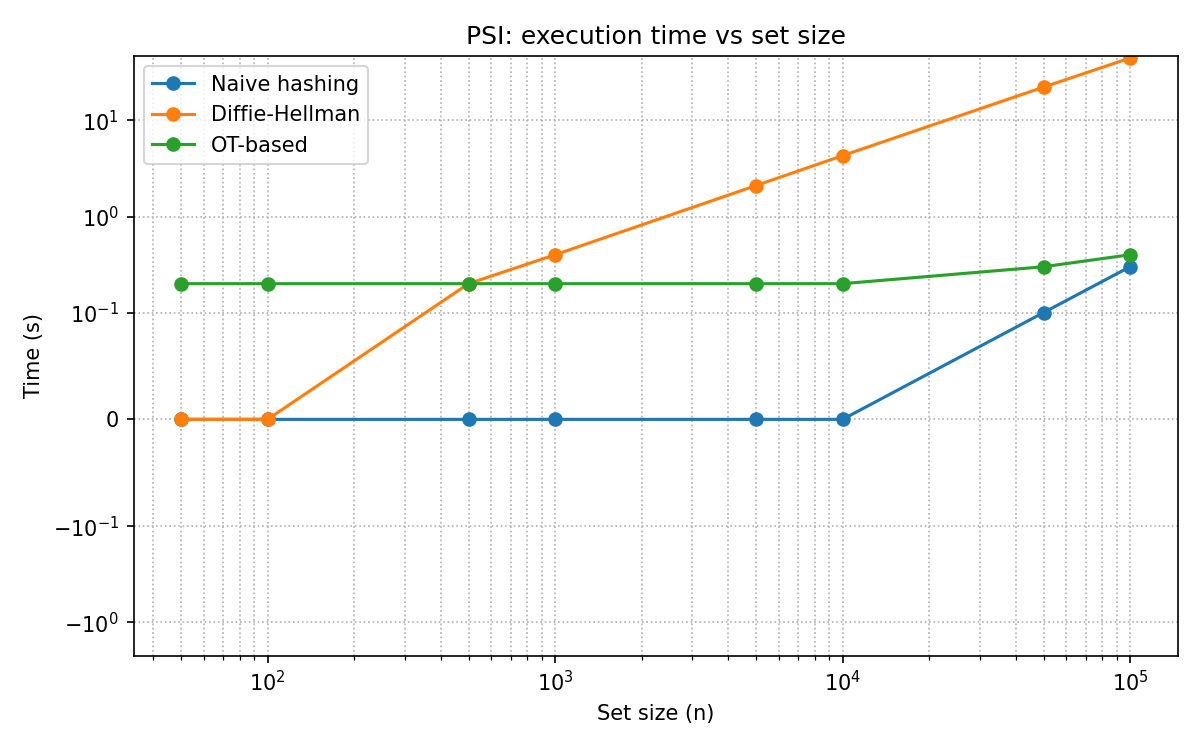
\includegraphics[width=0.95\textwidth]{pictures/bench_time_vs_n.png}
\caption{Tempo de execução em função de $n$ para os três protocolos benchmarkados.}
\label{fig:time_vs_n}
\end{figure}

\begin{figure}[H]
\centering
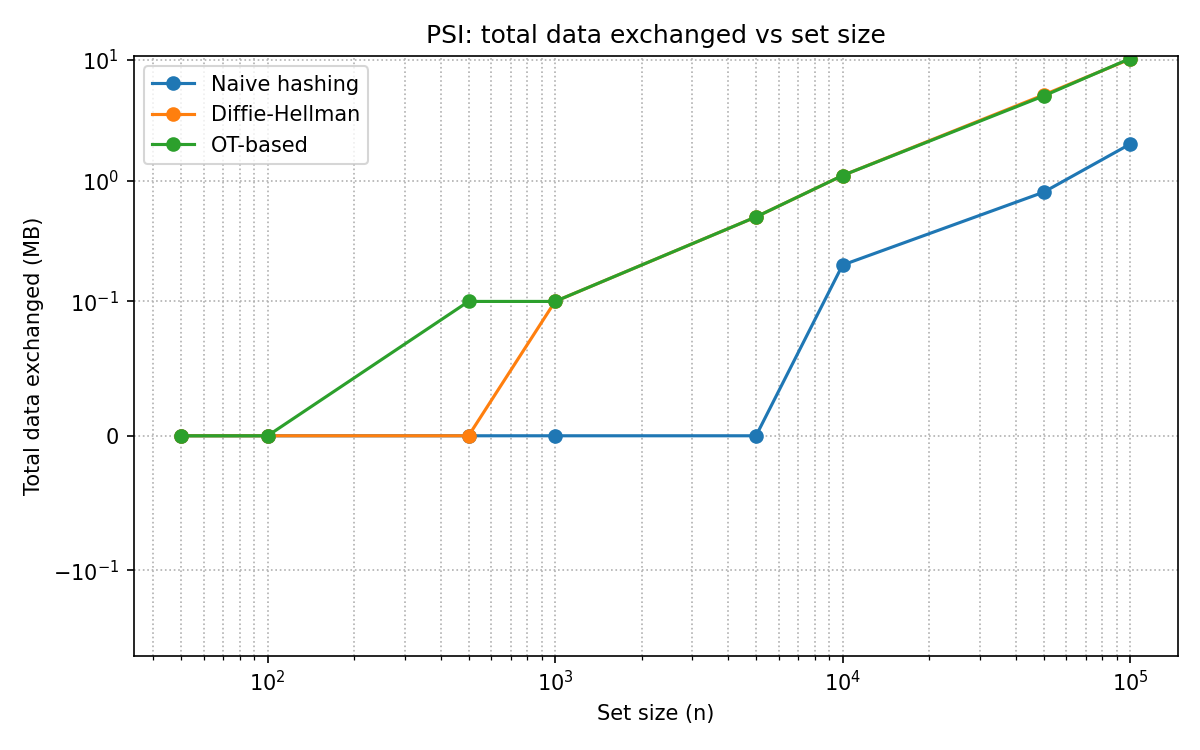
\includegraphics[width=0.95\textwidth]{pictures/bench_data_vs_n.png}
\caption{Dados totais trocados (sent + recv) em função de $n$.}
\label{fig:data_vs_n}
\end{figure}

\subsection{Análise dos Resultados}
\label{sec:bench_analise}

A Tabela~\ref{tab:bench} e as Figuras~\ref{fig:time_vs_n} e~\ref{fig:data_vs_n} permitem distinguir três regimes claramente diferentes em função do protocolo, e revelam como os custos teóricos discutidos na Secção~\ref{sec:step1} se materializam empiricamente em volume de dados e tempo de execução.

O protocolo \emph{naive} confirma o seu papel de baseline: tanto o tempo como o volume de dados crescem de forma aproximadamente linear em $n$, mas com constantes tão baixas que para $n = 100\,000$ o protocolo termina em apenas 0.3 segundos e troca cerca de 2 MB no total. Estes valores são mais de duas ordens de grandeza inferiores aos dos protocolos seguros para o mesmo $n$, o que reforça que o naive é, do ponto de vista exclusivamente de eficiência, virtualmente óptimo. As implicações de segurança permanecem, no entanto, as discutidas no Step~2 e impedem o seu uso fora de cenários muito específicos.

O protocolo de \emph{Diffie-Hellman} apresenta o crescimento mais acentuado em tempo: passa de 0.4 s para $n = 1\,000$ a 44.6 s para $n = 100\,000$, com uma curva praticamente linear na Figura~\ref{fig:time_vs_n}. Este comportamento é a manifestação directa das $2n$ exponenciações modulares por parte exigidas pelo protocolo: cada elemento adicional impõe um custo computacional fixo na ordem de centenas de microssegundos, que se acumula linearmente. O volume de dados, em contrapartida, mantém-se moderado (10.1 MB para $n = 100\,000$) e proporcional a $n$, dado que cada elemento corresponde a um único elemento do grupo cíclico.

O protocolo baseado em \emph{Oblivious Transfer} exibe o comportamento qualitativamente mais distinto: o tempo de execução mantém-se praticamente constante e abaixo de meio segundo em toda a gama testada (0.2 s para $n = 50$ e 0.4 s para $n = 100\,000$). Este perfil decorre directamente da estrutura do protocolo, que paga um overhead fixo correspondente à fase de \emph{base OTs} e à montagem do canal de OT extension; uma vez pago esse custo, cada elemento adicional é processado por primitivas simétricas extremamente rápidas. O custo em comunicação, por sua vez, cresce linearmente, atingindo 10.2 MB para $n = 100\,000$, valor próximo do DH mas com perfil distinto: domina para $n$ pequenos (em que é quase inteiramente custo fixo) e amortiza-se à medida que $n$ aumenta.

Da intersecção destes três comportamentos resultam dois pontos de cruzamento relevantes. Em \textbf{tempo}, o DH só é competitivo com o OT para $n$ na ordem das centenas: a partir de $n \approx 1\,000$, em que o DH demora 0.4 s e o OT continua nos 0.2 s, o OT torna-se estritamente preferível, e a vantagem agrava-se rapidamente até ser de cerca de duas ordens de grandeza para $n = 100\,000$. Em \textbf{volume de dados}, os dois protocolos seguros são essencialmente equivalentes para $n$ grande (ambos rondam os 10 MB para $n = 100\,000$), com o OT a ser ligeiramente mais pesado para $n$ pequenos devido ao overhead inicial.

A consequência prática é uma regra de selecção orientada pelo recurso mais escasso. Em ambientes constrangidos em CPU mas com largura de banda abundante, o OT é claramente preferível, dado que o seu tempo praticamente constante o torna o único candidato viável para conjuntos com dezenas de milhares de elementos. Em ambientes muito constrangidos em comunicação, mas com CPU disponível e $n$ moderado, o DH continua a fazer sentido, sobretudo se a sua simplicidade conceptual e a ausência de fase de inicialização forem desejáveis. Para conjuntos pequenos (centenas ou poucos milhares), a escolha entre DH e OT é essencialmente neutra em desempenho, e os critérios de implementação ou de modelo de adversário ganham preponderância sobre o custo bruto.


% =============================================================
%  STEP 4: APLICAÇÃO A DATASET PRÓPRIO
% =============================================================
\section{Aplicação a Dataset Próprio: Liked Songs do Spotify}
\label{sec:step4}

\subsection{Caso de Uso e Datasets}
\label{sec:step4_caso}

O cenário escolhido para esta etapa foi descobrir as músicas em comum entre as playlists \emph{Liked Songs} de Spotify dos dois autores, sem que nenhum revelasse ao outro o resto da sua biblioteca musical. Embora a sensibilidade desta informação seja menor que, por exemplo, contactos ou histórico de navegação, o exercício permite aplicar PSI a um caso real, com volumes da ordem das centenas, e validar empiricamente o protocolo escolhido. Cada autor exportou as suas Liked Songs para CSV recorrendo à ferramenta \emph{Exportify}, obtendo-se 579 entradas para o Artur e 601 entradas para o Tiago.

O \texttt{Track URI} do Spotify (formato \texttt{spotify:track:<id>}, com 22 caracteres em base62) constitui um identificador único, estável e independente de localização ou idioma, sendo por isso o atributo escolhido como elemento de input para o PSI. Foi escrito um pequeno script de extracção que lê o CSV exportado e produz apenas a lista de IDs, descartando metadados como nome da faixa, álbum, artista, data de adição ou \emph{features} áudio. Esta informação não é necessária para o cálculo da intersecção e a sua exclusão reduz a superfície de privacidade.

\subsection{Justificação do Protocolo}
\label{sec:step4_proto}

A escolha do protocolo decorre directamente da análise do Step~3. Para conjuntos da ordem das centenas, naive e DH são competitivos em tempo absoluto, mas o naive foi descartado por insegurança: o domínio dos Track IDs do Spotify é público e finito, pelo que um atacante que observasse os hashes truncados poderia compará\-los contra o catálogo público e re\-identificar trivialmente todas as faixas de cada parte. O DH oferece segurança adequada mas escala mal em CPU para tamanhos maiores (cerca de 2\,s para 5k elementos no benchmark). O \textbf{OT\-based (-p 3)} foi seleccionado por combinar segurança forte~\cite{pinkas2016scalable} com tempo praticamente constante e custo de comunicação aceitável para esta gama de $n$ (cerca de 0.1\,MB para 1k elementos). É também o protocolo de eleição se a aplicação fosse mais tarde estendida a milhares de utilizadores.

\subsection{Execução e Resultado}
\label{sec:step4_exec}

A biblioteca exige $n$ igual em ambos os lados (mesma limitação registada no ponto~6 do Step~2). A lista do Artur foi paddada de 579 para 601 entradas com 22 IDs falsos de 22 caracteres prefixados com \texttt{FAKE}. Estes IDs nunca colidem com IDs reais, uma vez que todos os IDs reais do Spotify usam apenas o alfabeto base62 e o prefixo \texttt{FAKE} fica fora desse alfabeto, pelo que não introduzem falsos positivos. Cada autor executou então a sua instância: o Artur com \texttt{./demo.exe -r 0 -p 3 -f <ids\_artur>} e o Tiago com \texttt{./demo.exe -r 1 -p 3 -f <ids\_tiago>}.

O output do protocolo reportou \textbf{2 elementos intersectados}, validados a posteriori contra a intersecção em plaintext (\texttt{comm -12} sobre os dois ficheiros de IDs ordenados):

\begin{itemize}
  \item \texttt{4nKRZAONxGgcKCMin730Ai}: \emph{33 Max Verstappen} (Carte Blanq; Nils Van Zandt; Maxx Power)
  \item \texttt{63T7DJ1AFDD6Bn8VzG6JE8}: \emph{Paint It, Black} (The Rolling Stones)
\end{itemize}

Cada parte aprende apenas estes 2 IDs; as restantes 577 e 599 entradas permanecem privadas. A correspondência entre o ID e o título da faixa foi reconstruída \emph{a posteriori} por cada autor, consultando o seu próprio CSV, uma vez que o protocolo só transmite os IDs. A Figura~\ref{fig:step4_ot} mostra o output do cliente (\texttt{-r 1}) e permite confirmar a configuração concreta do protocolo para este caso: 601 elementos hashados em palavras de 8 bytes, 722 \emph{bins} e 722 OTs efectuadas, com \texttt{maskbitlen = 64}.

\begin{figure}[H]
\centering
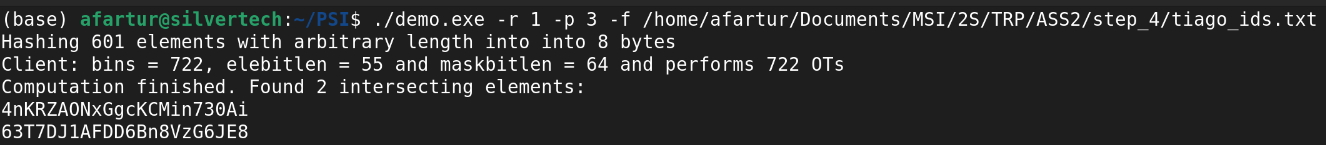
\includegraphics[width=0.95\textwidth]{pictures/step4_ot.png}
\caption{Output do cliente do protocolo OT-based aplicado às listas de Track IDs do Spotify, com a intersecção de 2 elementos correctamente identificada.}
\label{fig:step4_ot}
\end{figure}

\subsection{Considerações de Privacidade}
\label{sec:step4_priv}

A escolha de PSI como mecanismo para este caso de uso justifica-se directamente pelo princípio da minimização de divulgação. A alternativa trivial seria cada autor partilhar a sua lista de Track IDs com o outro e calcular a intersecção em claro, mas essa abordagem revelaria à contraparte a totalidade da biblioteca musical de cada um, ou seja, 599 e 577 elementos que não pertencem à intersecção e que não são necessários para o objectivo do protocolo. PSI substitui essa partilha total por uma partilha estritamente limitada à intersecção, neste caso 2 IDs, sem que qualquer informação sobre os restantes elementos transite entre as partes. Mesmo num cenário em que a sensibilidade da informação musical seja considerada baixa, a aplicação do princípio é metodologicamente correcta e prepara o protocolo para extensões a domínios onde a sensibilidade seja crítica, como contactos pessoais, histórico clínico ou identificadores de autenticação.

Permanecem, contudo, várias fugas de informação que não são eliminadas pelo protocolo e que importa enumerar. Em primeiro lugar, o tamanho dos conjuntos é necessariamente revelado: a biblioteca exige que ambos os lados forneçam $n$ idêntico, pelo que cada parte aprende que a contraparte possui pelo menos $n$ elementos. O recurso a \emph{padding} com IDs falsos prefixados com \texttt{FAKE} garante que esses elementos não introduzem falsos positivos na intersecção, mas não esconde a cardinalidade real, que continua a ser inferível através de canais laterais (por exemplo, o tempo de leitura do ficheiro de input ou o conhecimento informal de quanta música a contraparte tipicamente ouve). Numa aplicação verdadeiramente sensível, esta fuga teria de ser mitigada com técnicas adicionais como \emph{padding} aleatório a um valor superior ao máximo plausível para ambas as partes.

Em segundo lugar, o protocolo revela à contraparte não só os elementos da intersecção mas também a sua cardinalidade, o que permite inferências do género ``a tua lista contém este conjunto de músicas''. Como o domínio dos Track IDs do Spotify é público e enumerável, cada ID na intersecção pode ser convertido por qualquer das partes no nome da faixa por simples consulta ao catálogo, exactamente como qualquer atacante o faria. Esta propriedade é inerente ao próprio conceito de PSI e não constitui uma fragilidade do protocolo, mas merece registo: aprender que um determinado utilizador gosta de ``Paint It, Black'' é, em si, informação pessoal, mesmo que limitada ao subconjunto comum.

Em terceiro lugar, a inferência sobre o que \emph{não} está na intersecção também é possível em casos extremos. Se uma das partes souber, ou suspeitar, que um determinado elemento pertence ao seu próprio conjunto e o resultado do PSI o excluir da intersecção, conclui imediatamente que esse elemento não está no conjunto da contraparte. Esta fuga é uma consequência inevitável do output correcto do PSI e demonstra que mesmo um protocolo perfeitamente executado fornece informação além da intersecção, sempre que o atacante combine o output com conhecimento prévio sobre o seu próprio conjunto.

Por fim, é relevante notar que o modelo de segurança garantido pelo protocolo OT-based é semi-honesto. Caso uma das partes seja activamente maliciosa, pode forjar IDs com a expectativa de que apareçam na intersecção e, dessa forma, sondar o conjunto da contraparte. Este vector é mitigado, no caso concreto deste trabalho, pela ausência de incentivos significativos para tal comportamento entre os dois autores, mas seria uma preocupação séria em aplicações reais com adversários estranhos, exigindo o recurso a versões maliciosamente seguras de PSI ou a mecanismos adicionais de autenticação dos inputs.


% =============================================================
%  CONCLUSÃO
% =============================================================
\section{Conclusão}
\label{sec:conclusao}

Este trabalho permitiu estudar e comparar quatro protocolos de \emph{Private Set Intersection} representativos de pontos diferentes do espaço de compromissos entre eficiência, escalabilidade e garantias criptográficas, e validar empiricamente os respectivos trade-offs anunciados na literatura. A combinação da análise teórica do Step~1 com as experimentações controladas do Step~2 e os benchmarks do Step~3 ofereceu uma visão coerente e mensurável do comportamento de cada protocolo, que culminou na sua aplicação prática a um caso de uso real no Step~4.

O protocolo \emph{naive hashing} confirmou-se como o mais eficiente em qualquer dimensão de desempenho, mas as capturas em Wireshark e a análise dos pontos 4 e 7 do Step~2 demonstraram com clareza que o seu uso em domínios públicos e enumeráveis, como aplicações Android ou identificadores de música, equivale a uma divulgação quase total dos elementos. A truncagem agressiva dos hashes a 6 bytes, combinada com a ausência de qualquer segredo partilhado, torna trivial a re-identificação por dicionário. O protocolo \emph{server-aided}, embora reduza a interacção a uma única ronda cliente-servidor, herda essas mesmas fragilidades na implementação observada e introduz um ponto único de falha que torna a sua utilização desaconselhável fora de contextos onde a hipótese de não-colusão entre servidor e clientes seja credível e o ganho de escalabilidade compense efectivamente os riscos.

Os protocolos baseados em \emph{Diffie-Hellman} e em \emph{Oblivious Transfer} oferecem garantias de privacidade substancialmente superiores e cobrem regimes operacionais complementares. O DH é simples, sem fase de inicialização e adequado a conjuntos pequenos ou a ambientes onde a CPU é abundante e a largura de banda é o recurso crítico, mas escala mal: a 100\,000 elementos demora 44.6 s contra os 0.4 s do OT. O protocolo OT-based, à custa de uma maior complexidade de implementação e de um overhead fixo de comunicação que penaliza conjuntos pequenos, mantém um tempo de execução praticamente constante em toda a gama testada e impõe-se como a escolha natural para volumes médios e grandes. A escolha entre os dois é, na prática, uma função do recurso mais escasso e do tamanho expectável dos conjuntos.

A aplicabilidade prática deste raciocínio ficou demonstrada no Step~4, onde o protocolo OT-based foi usado para calcular a intersecção entre as bibliotecas \emph{Liked Songs} de Spotify dos dois autores. O protocolo identificou correctamente as 2 faixas comuns entre 579 e 601 entradas, sem que qualquer outro elemento das duas bibliotecas tivesse sido revelado, ilustrando o ganho concreto que PSI oferece face a uma partilha em claro. As considerações de privacidade da Secção~\ref{sec:step4_priv} mostraram, no entanto, que mesmo um protocolo correctamente executado deixa fugas residuais (cardinalidade dos conjuntos, possibilidade de inferência sobre o complemento e dependência do modelo semi-honesto), que devem ser ponderadas em qualquer aplicação real e que abrem direcções naturais de continuação do trabalho, nomeadamente a adopção de versões maliciosamente seguras de PSI e o uso de \emph{padding} aleatório para esconder cardinalidades. As limitações da biblioteca utilizada, em particular o requisito de $n$ idêntico em ambos os lados e a ausência de uma defesa nativa contra adversários activos, tornam-se evidentes neste tipo de aplicação e reforçam a necessidade de continuar a desenvolver implementações de PSI orientadas a casos de uso reais.
